% Séquence 1 : Les nombres relatifs
\setseqtitle{Les nombres relatifs}
\chapter{Les nombres relatifs}

\begin{objectifsbox}
À l'issue de la séquence, l'élève sera capable de :
\begin{itemize}
\item Représenter et comparer des nombres relatifs sur une droite graduée
\item Calculer la distance à zéro d'un nombre relatif
\item Additionner et soustraire des nombres relatifs
\item Multiplier et diviser des nombres relatifs en appliquant la règle des signes
\item Généraliser la règle des signes pour plusieurs facteurs
\item Identifier et utiliser les nombres inverses
\item Résoudre des problèmes utilisant les nombres relatifs
\item Calculer des expressions numériques avec enchaînements d'opérations
\end{itemize}
\end{objectifsbox}

\section{Introduction aux nombres relatifs}

Les nombres relatifs sont utilisés dans de nombreuses situations de la vie quotidienne :
\begin{itemize}[label = \textbullet]
\item Mesurer des températures (température positive ou négative)
\item Mesurer des altitudes (au-dessus ou en dessous du niveau de la mer)
\item Gérer des soldes bancaires (crédit ou dette)
\item Se repérer dans le temps (avant ou après un événement)
\end{itemize}

Ils nous permettent de décrire des quantités qui peuvent être positives (au-dessus de zéro) ou négatives (en dessous de zéro).

\section{Définition et représentation}

\begin{definitionbox}
Un \textbf{nombre relatif} est un nombre qui peut être positif, négatif ou nul.
\end{definitionbox}

\subsection{La droite graduée}

Un nombre relatif est repéré par son signe (+ ou -) et sa distance à zéro.

Sur une droite graduée, le point de référence est l'origine (0).

\begin{proprietebox}
\begin{itemize}[label = \textbullet]
\item Les nombres positifs sont à droite de 0.
\item Les nombres négatifs sont à gauche de 0.
\item Plus un nombre est à droite, plus il est grand.
\item Plus un nombre est à gauche, plus il est petit.
\end{itemize}
\end{proprietebox}

\begin{examplebox}
Sur la droite graduée ci-dessous, on peut voir que $-3 < -1 < 0 < 2 < 5$

\begin{center}
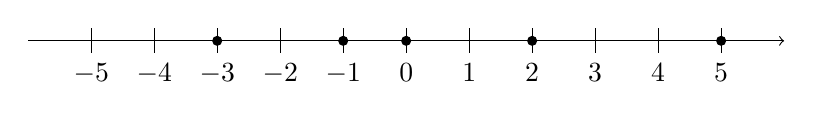
\begin{tikzpicture}[scale=0.8]
\draw[->] (-6,0) -- (6,0);
\foreach \x in {-5,-4,-3,-2,-1,0,1,2,3,4,5}
    \draw (\x,0.2) -- (\x,-0.2) node[below] {$\x$};
\draw[fill=black] (-3,0) circle (2pt);
\draw[fill=black] (-1,0) circle (2pt);
\draw[fill=black] (0,0) circle (2pt);
\draw[fill=black] (2,0) circle (2pt);
\draw[fill=black] (5,0) circle (2pt);
\end{tikzpicture}
\end{center}
\end{examplebox}

\subsection{Distance à zéro}

\begin{definitionbox}
La \textbf{distance à zéro} d'un nombre relatif est la distance qui le sépare de 0 sur la droite graduée. C'est un nombre \textbf{toujours positif}.
\end{definitionbox}

\begin{examplebox}
\begin{itemize}[label = \textbullet]
\item La distance à zéro de +6 est \trous{2cm}
\item La distance à zéro de -4,5 est \trous{2cm}
\item La distance à zéro de 0 est \trous{2cm}
\end{itemize}
\end{examplebox}

\subsection{Nombres opposés}

\begin{definitionbox}
Deux nombres sont \textbf{opposés} s'ils ont la \textbf{même distance à zéro} mais des \textbf{signes différents}. Leur somme est toujours égale à 0.
\end{definitionbox}

\begin{examplebox}
\begin{itemize}[label = \textbullet]
\item L'opposé de +7 est \trous{2cm}
\item L'opposé de -2,3 est \trous{2cm}
\item L'opposé de 0 est \trous{2cm}
\end{itemize}
\end{examplebox}

\section{Addition et soustraction}
\subsection{Addition de nombres relatifs}
\begin{proprietebox}
Pour \textbf{additionner deux nombres de MÊME SIGNE :}
\begin{itemize}[label = \textbullet]
\item On \textbf{garde le signe commun}.
\item On \textbf{additionne} leurs distances à zéro.
\end{itemize}
\end{proprietebox}

\begin{examplebox}
\begin{align*}
(+5) + (+9) &= \trous{2cm} \quad \text{(Le signe commun est +, et } 5 + 9 = 14\text{)} \\
(-7) + (-3) &= \trous{2cm} \quad \text{(Le signe commun est -, et } 7 + 3 = 10\text{)} \\
(-1,5) + (-4) &= \trous{2cm}
\end{align*}
\end{examplebox}

\begin{proprietebox}
Pour \textbf{additionner deux nombres de SIGNE DIFFÉRENT :}
\begin{itemize}[label = \textbullet]
\item On \textbf{garde le signe du nombre qui a la plus grande distance à zéro}.
\item On \textbf{soustrait} la plus petite distance à zéro de la plus grande.
\end{itemize}
\end{proprietebox}

\begin{examplebox}
\begin{align*}
(+8) + (-3) &= \trous{2cm} \quad \text{(8 > 3, donc on garde le signe + et } 8 - 3 = 5\text{)} \\
(-6) + (+9) &= \trous{2cm} \quad \text{(9 > 6, donc on garde le signe + et } 9 - 6 = 3\text{)} \\
(+2,5) + (-7) &= \trous{2cm} \quad \text{(7 > 2,5, donc on garde le signe - et } 7 - 2,5 = 4,5\text{)}
\end{align*}
\end{examplebox}

\subsection{Soustraction de nombres relatifs}

\begin{proprietebox}
\textbf{Soustraire un nombre relatif, c'est ajouter son opposé :}
$$a - b = a + (-b)$$
\end{proprietebox}

\begin{examplebox}
\begin{align*}
(+5) - (+3) &= \trous{2.5cm} = \trous{2cm} \\
(+4) - (-2) &= \trous{2.5cm} = \trous{2cm} \\
(-7) - (+1) &= \trous{2.5cm} = \trous{2cm} \\
(-3) - (-5) &= \trous{2.5cm} = \trous{2cm}
\end{align*}
\end{examplebox}

\section{Multiplication et division}

\subsection{Règle des signes}

\begin{proprietebox}
\textbf{Règle des signes pour la multiplication et la division :}
\begin{itemize}[label = \textbullet]
\item Le produit (ou quotient) de deux nombres de \textbf{même signe} est \textbf{positif}
\item Le produit (ou quotient) de deux nombres de \textbf{signes contraires} est \textbf{négatif}
\end{itemize}
\end{proprietebox}

\begin{examplebox}
\begin{minipage}[t]{0.48\textwidth}
\textbf{Multiplication :}
\begin{align*}
(+4) \times (+3) &= \trous{2cm} \\
(-5) \times (-2) &= \trous{2cm} \\
(+6) \times (-3) &= \trous{2cm} \\
(-7) \times (+4) &= \trous{2cm}
\end{align*}
\end{minipage}
\hfill
\begin{minipage}[t]{0.48\textwidth}
\textbf{Division :}
\begin{align*}
(+15) \div (+3) &= \trous{2cm} \\
(-20) \div (-4) &= \trous{2cm} \\
(+24) \div (-6) &= \trous{2cm} \\
(-35) \div (+7) &= \trous{2cm}
\end{align*}
\end{minipage}
\end{examplebox}

\subsection{Généralisation de la règle des signes}
\begin{proprietebox}
\textbf{Produit de plusieurs nombres relatifs :}
Le produit de plusieurs nombres relatifs sera de signe :
\begin{itemize}[label = \textbullet]
\item \textbf{positif} s'il y a un nombre \textbf{pair} de facteurs négatifs
\item \textbf{négatif} s'il y a un nombre \textbf{impair} de facteurs négatifs
\end{itemize}
\end{proprietebox}

\begin{examplebox}
\textbf{Déterminer le signe des produits suivants :}

\begin{align*}
A &= (-2) \times (+3) \times (-4) \times (-1) \\
B &= (-1) \times (-2) \times (-3) \times (-4) \\
C &= (+5) \times (-6) \times (+7) \times (-8) \times (-9)
\end{align*}

\begin{itemize}[label = \textbullet]
\item $A$ est \trous{2.5cm} car il y a \trous{1.5cm} facteurs négatifs et \trous{1.5cm} est un nombre impair.
\item $B$ est \trous{2.5cm} car il y a \trous{1.5cm} facteurs négatifs et \trous{1.5cm} est un nombre pair.
\item $C$ est \trous{2.5cm} car il y a \trous{1.5cm} facteurs négatifs et \trous{1.5cm} est un nombre impair.
\end{itemize}
\end{examplebox}

\subsection{Nombres inverses}
\begin{definitionbox}
Deux nombres relatifs sont des \textbf{nombres inverses} si leur produit est égal à 1.

Soit $a$ et $b$ deux nombres relatifs. $a$ et $b$ sont dits « inverses » si et seulement si $a \times b = 1$.
\end{definitionbox}

\begin{examplebox}
\begin{itemize}[label = \textbullet]
\item L'inverse de 5 est \trous{1cm} car $5 \times \trous{1cm} = 1$
\item L'inverse de $-\frac{2}{3}$ est \trous{1cm} car $-\frac{2}{3} \times$ \trous{1cm} = 1
\item L'inverse de -4 est \trous{1cm} car $-4 \times$ \trous{1cm} = 1
\end{itemize}
\end{examplebox}

\subsection{Simplification des écritures}
\begin{remarkbox}
\textbf{Conventions d'écriture :}
\begin{itemize}[label = \textbullet]
\item On peut écrire $+5$ au lieu de $(+5)$
\item On peut écrire $-3$ au lieu de $(-3)$
\item Le signe $+$ peut être omis pour les nombres positifs : $5$ au lieu de $+5$
\item Le signe $-$ ne peut jamais être omis pour les nombres négatifs
\end{itemize}
\end{remarkbox}

\section{Expressions numériques et enchaînements d'opérations}
\begin{methodebox}
\textbf{Pour calculer une expression numérique :}
\begin{enumerate}[label = \arabic*)]
\item On effectue en premier les calculs dans les \textbf{parenthèses les plus intérieures}
\item On calcule les \textbf{puissances} éventuelles
\item On effectue ensuite les \textbf{multiplications et divisions} avant les additions et soustractions
\item Si plusieurs multiplications/divisions se suivent, on calcule dans le \textbf{sens de la lecture}
\item Si plusieurs additions/soustractions se suivent, on calcule dans le \textbf{sens de la lecture}
\end{enumerate}
\end{methodebox}

\begin{examplebox}
\textbf{Calculer les expressions suivantes :}

\noindent
\begin{minipage}[t]{0.48\textwidth}
\begin{align*}
A &= 5 + 3 \times (-2) \\
  &= \trous{2.5cm} \\
  &= \trous{2.5cm}
\end{align*}
\end{minipage}
\hfill
\begin{minipage}[t]{0.48\textwidth}
\begin{align*}
B &= (-8) \div 2 + 3 \times (-1) \\
  &= \trous{2.5cm} \\
  &= \trous{2.5cm}
\end{align*}
\end{minipage}

\vspace{1em}

\noindent
\begin{minipage}[t]{0.48\textwidth}
\begin{align*}
C &= [(-6) + 4] \times (-2) \\
  &= \trous{2.5cm} \\
  &= \trous{2.5cm}
\end{align*}
\end{minipage}
\hfill
\begin{minipage}[t]{0.48\textwidth}
\begin{align*}
D &= 12 \div (-3) \times 2 \\
  &= \trous{2.5cm} \\
  &= \trous{2.5cm}
\end{align*}
\end{minipage}
\end{examplebox}

\section{Exercices d'application}

\begin{exercisebox}
\textbf{Exercice 1 :} Représenter et comparer

\begin{enumerate}[label=\alph*)]
\item Représenter sur une droite graduée les nombres : $-4$ ; $+2$ ; $-1$ ; $+5$ ; $0$ ; $-3$
\item Ranger ces nombres dans l'ordre croissant
\item Donner la distance à zéro de chaque nombre
\end{enumerate}

\textbf{Exercice 2 :} Calculs avec les nombres relatifs

Calculer les expressions suivantes :
\begin{enumerate}[label=\alph*)]
	\item $A = (+7) + (-3) + (+2)$
	\item $B = (-5) + (+8) + (-1)$
	\item $C = (+4) - (-6) + (-2)$
	\item $D = (-3) - (+5) - (-2)$
\end{enumerate}

\textbf{Exercice 3 :} Multiplication et division

Calculer :
\begin{enumerate}[label=\alph*)]
	\item $E = (+6) \times (-4)$
	\item $F = (-8) \times (-3)$
	\item $G = (+24) \div (-6)$
	\item $H = (-35) \div (-7)$
\end{enumerate}

\textbf{Exercice 4 :} Généralisation de la règle des signes

Déterminer le signe des produits suivants :
\begin{enumerate}[label=\alph*)]
	\item $I = (-2) \times (+3) \times (-4)$
	\item $J = (-1) \times (-2) \times (-3) \times (-4)$
	\item $K = (+5) \times (-6) \times (+7) \times (-8)$
\end{enumerate}

\textbf{Exercice 5 :} Expressions numériques

Calculer les expressions suivantes :
\begin{enumerate}[label=\alph*)]
	\item $L = 8 + 3 \times (-2)$
	\item $M = (-12) \div 3 + 2 \times (-1)$
	\item $N = [(-5) + 3] \times (-2)$
	\item $O = 15 \div (-3) \times 2$
\end{enumerate}

\textbf{Exercice 6 :} Problème

La température était de $-5\,\text{°C}$ le matin. Elle a augmenté de $+8\,\text{°C}$ dans la journée, puis baissé de $-3\,\text{°C}$ le soir.

\begin{enumerate}[label=\alph*)]
	\item Quelle était la température en fin de journée ?
	\item Quelle était la température le soir ?
\end{enumerate}
\end{exercisebox}

\begin{exercisebox}
\textbf{Exercice 7 :} Nombres inverses

Trouver l'inverse de chacun des nombres suivants :
\begin{enumerate}[label=\alph*)]
	\item $+6$
	\item $-\frac{1}{4}$
	\item $+2,5$
	\item $-\frac{3}{7}$
\end{enumerate}
\end{exercisebox}

